This is my short introduction.

\vspace{10px}
\noindent This is how you add references \cite{jupyterbook}, and a full reference as
\begin{enumerate}
    \item[$\star$] \printpublication{jupyterbook}
\end{enumerate}

\begin{figure}
\captionsetup{justification=centering, singlelinecheck=off}
\begin{center}
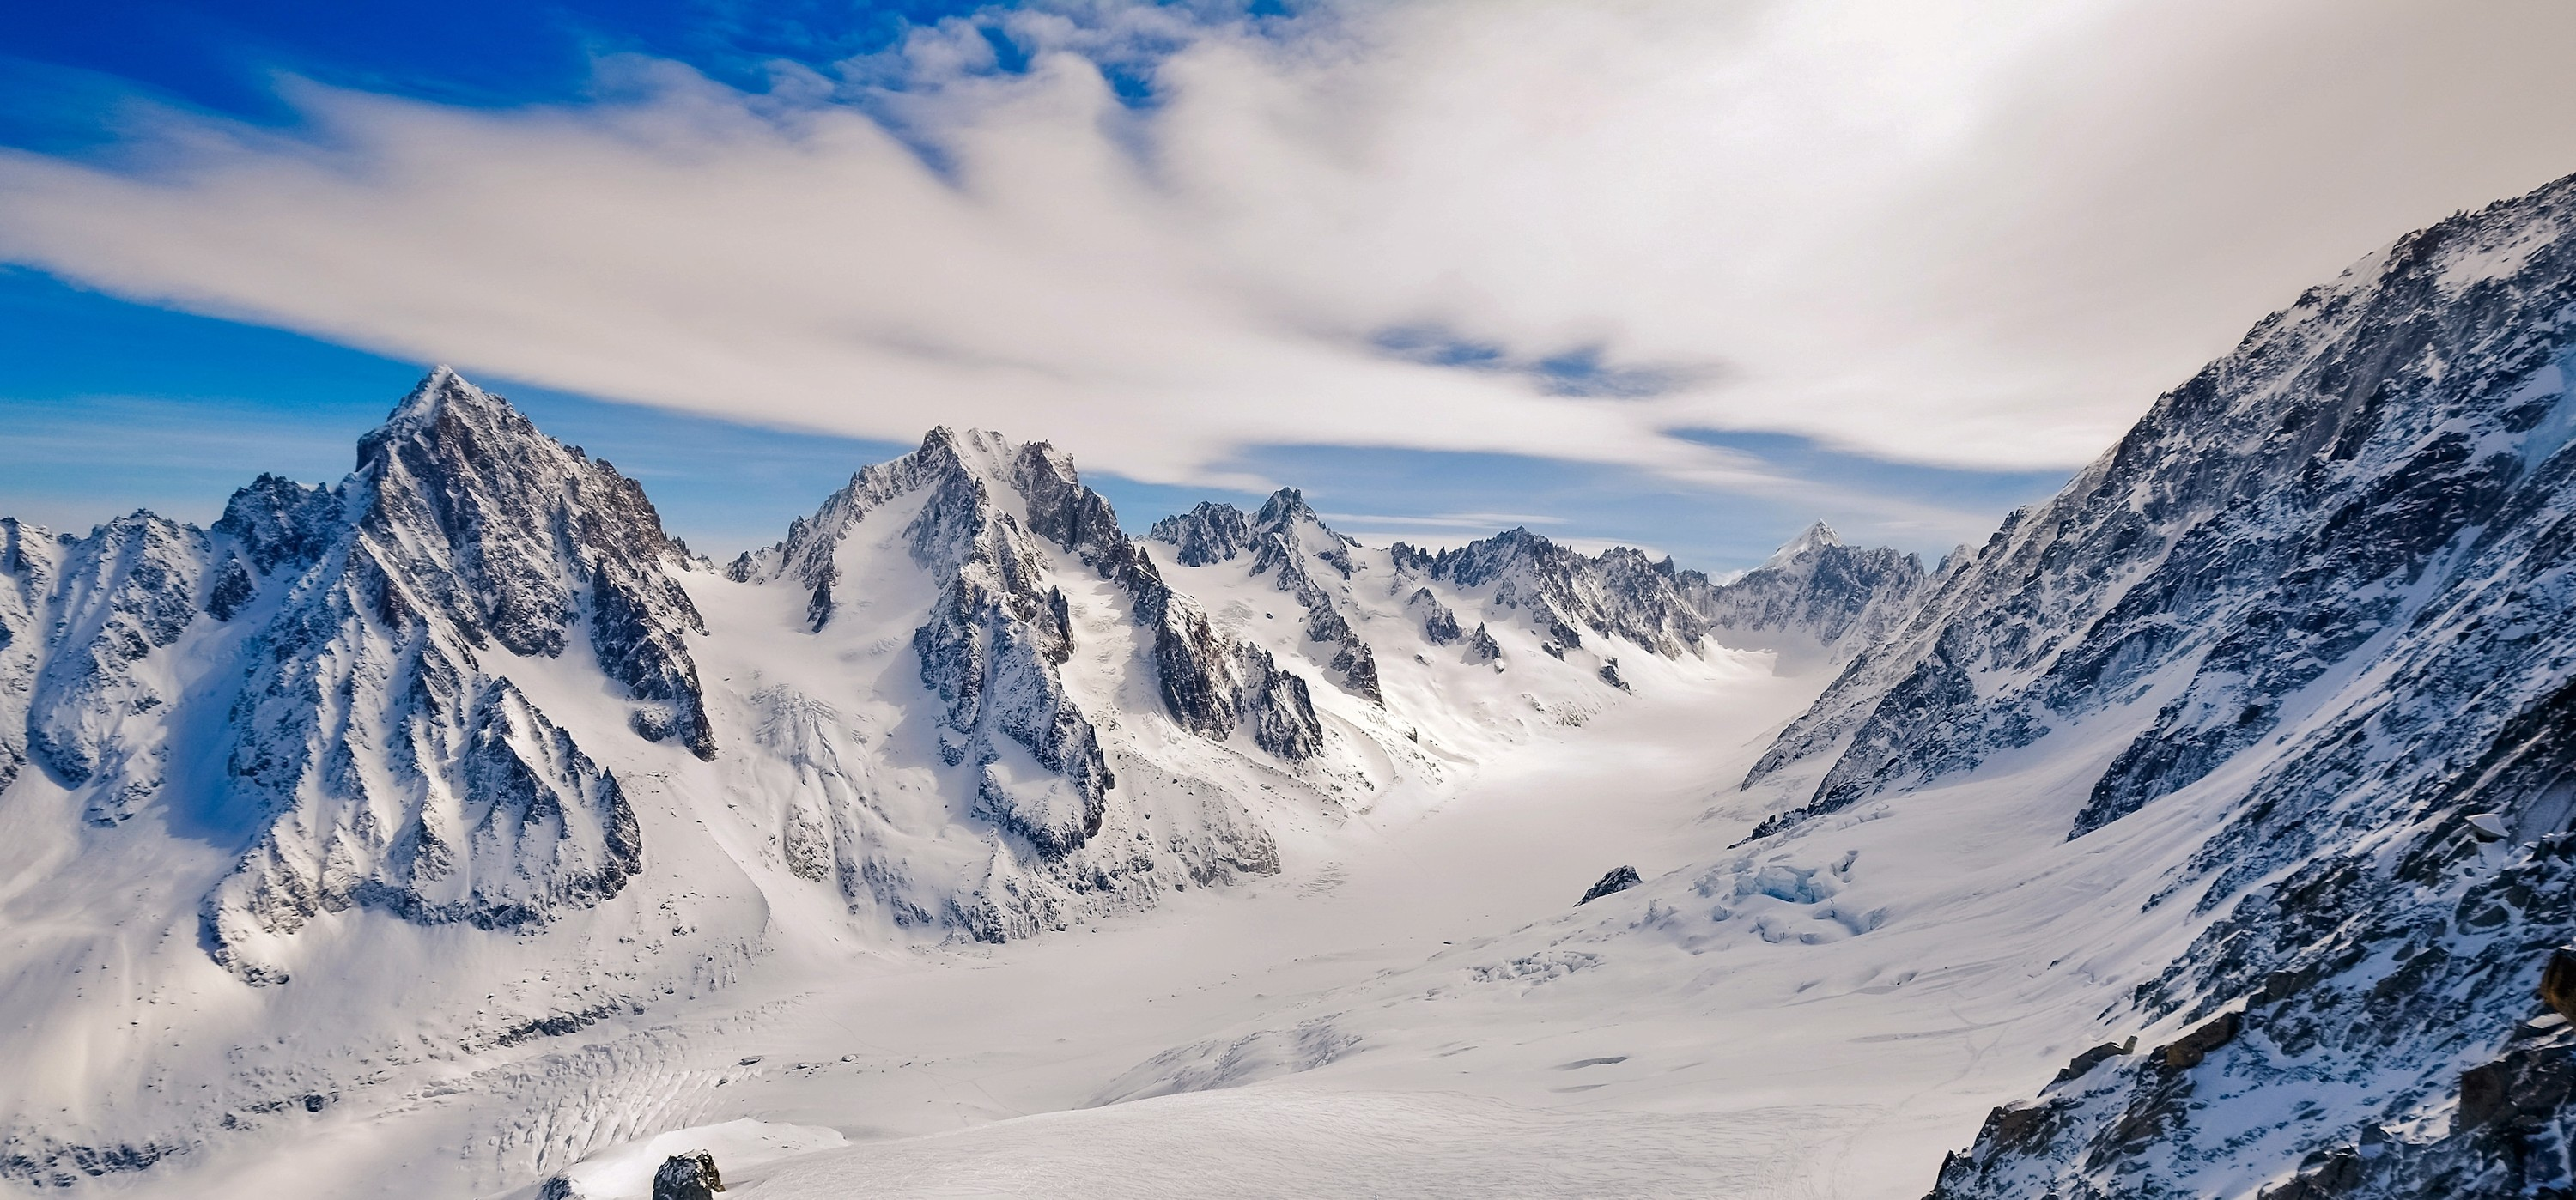
\includegraphics[width=\columnwidth]{figures/malchin.jpg}
\caption*{\textit{Malchin Peak, in the triple border between Mongolia, Russia, and China. Picture taken in 2018 by Facundo Sapienza.}}
\end{center}
\end{figure} 

\vspace{10px}
\noindent An hyperlink should show up with a nice format: \url{https://jupytearth.org/jupyter-resources/introduction/ecosystem.html}.

\vspace{10px}
\noindent And equation references, 
\begin{equation}
    E = mc^2
    \label{eq:emc2}
\end{equation}
should be nicely linked: Equation \eqref{eq:emc2}.

\vspace{10px}
\noindent This is how we make a roman enumerate:
\begin{enumerate}[label=(\roman*)]
    \item Option No1
    \item Option No2 
\end{enumerate}